\section{実験セットアップ}
図\ref{fig:ELPHSetup}に実験セットアップの概略図を示す。
$\SI{0.8}{GeV/c}$の陽電子をビームとして用いた。
T1、T2はトリガー検出器として使用したプラスチック・シンチレーターで、どちらも$\SI{10}{mm}\times\SI{10}{mm}\times\SI{5}{mm}$である。
輻射体として表\ref{table:Aerogel}に示す3つのエアロゲルを並べて使用した。
エアロゲルの中心から$\SI{1500}{mm}$離したところに九面鏡を設置し、ビームに対して$\ang{21.4}$傾けた方向に$\SI{1500}{mm}$離して設置した。
鏡はエアロゲルを設置する場所にレーザーを置き、鉛直・水平方向の光が鏡の中心にあたり検出面の中心に反射するようにアライメントを行った。
また、T1以外はチェレンコフ光以外を遮断するために遮光シートで覆った。
\begin{figure}
  \centering
  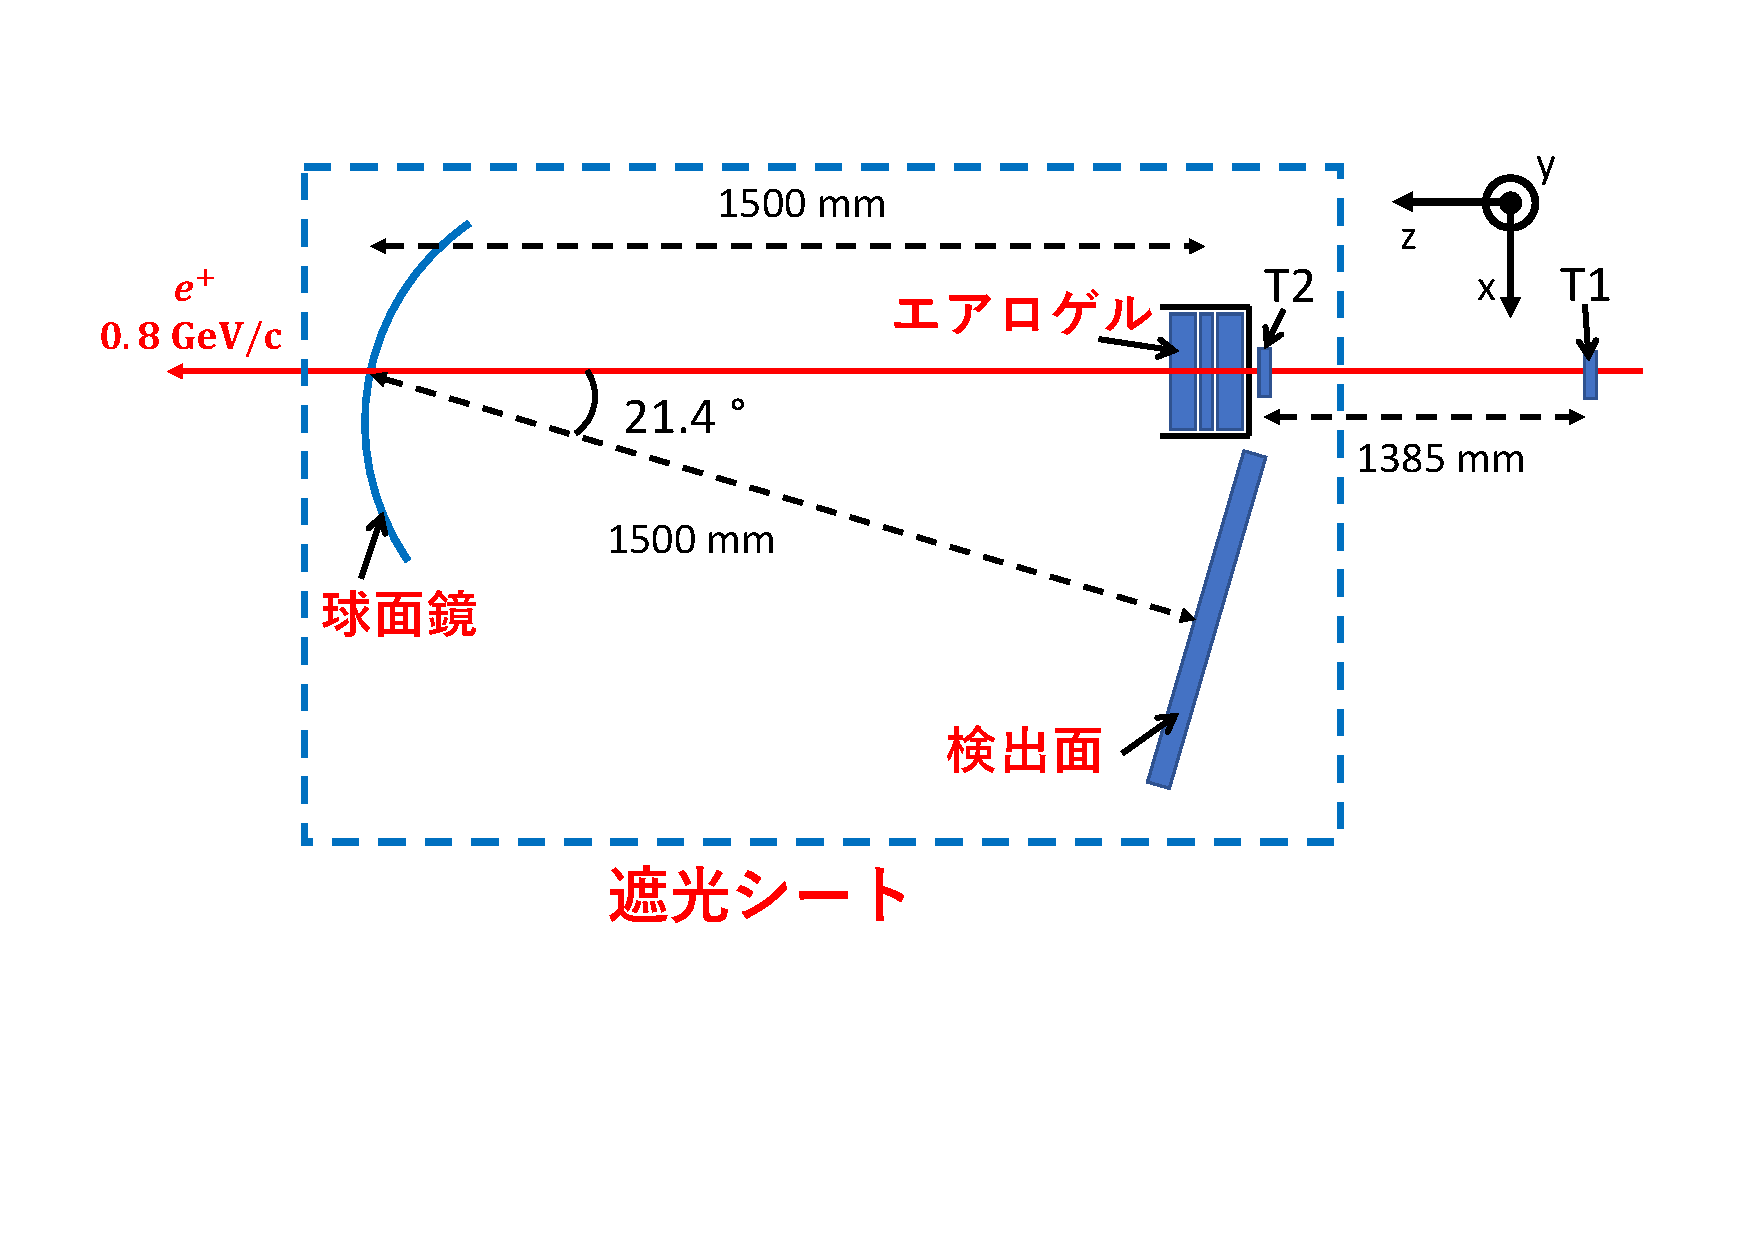
\includegraphics[width=15cm]{images/chapter3/ELPHSetup.pdf}
  \caption{実験セットアップを上から見た場合の概略図。}
  \label{fig:ELPHSetup}
\end{figure}

\subsection{検出面}
図\ref{fig:DetectorPlane}に実際の検出面の様子を示す。
今回のテスト実験では、用意できたMPPCの数では$\SI{1}{mm}\times\SI{1}{mm}$の検出面全体を覆うことはできなかったため、
$\SI{50}{mm}$コーンを使用する検出面ではチェレンコフリング周辺のみにコーン型ライトガイドとMPPCを配置した。
$\SI{30}{mm}$コーンを使用する検出面ではチェレンコフリング1周分を覆うことも難しかったため、飛地で配置している。
また、$\SI{30}{mm}$コーンでは、空気によるチェレンコフリングも測定できるように、中心部分にも検出面を配置している。

\begin{figure}
  \begin{tabular}{cc}
    \begin{minipage}[t]{0.45\hsize}
      \centering
      \includegraphics[keepaspectratio, scale=0.35, page=1]{images/chapter3/DetectorPlane.pdf}
    \end{minipage}
     &
    \begin{minipage}[t]{0.45\hsize}
      \centering
      \includegraphics[keepaspectratio, scale=0.35, page=2]{images/chapter3/DetectorPlane.pdf}
    \end{minipage}
  \end{tabular}
  \caption{実際の検出面の様子。左が$\SI{50}{mm}$コーンを使用した検出面、右が$\SI{30}{mm}$コーンを使用した検出面。
    $\SI{30}{mm}$コーンの写真は遮光後に撮ったもの。
  }
  \label{fig:DetectorPlane}
\end{figure}

\subsection{MPPC}
使用したMPPCの型番はS13360-6075CSで、
$\SI{50}{mm}$コーンの場合は216個、$\SI{30}{mm}$コーンの場合は中心の7個を含めて223個を使用した。
MPPCは降伏電圧($V_{BR}$)に個体差があるため、$V_{BR}$の順にグループ分けし、グループ毎に基盤に繋ぎ電圧をかけた。
外部電圧は降伏電圧が最大となるグループを基準に設定し、EASIROC内部でグループ毎のゲインが揃うように調節した。
閾値はグループ毎に調整し、$\SI{0.5}{p.e.}$の高さになるように設定した。


\subsection{エアロゲル}
使用したエアロゲルの写真を図\ref{fig:Aerogle}に、パラメータを表\ref{table:Aerogel}に示す。
実験では、複数のエアロゲルを組み合わせて厚さを変えながらデータを測定した。


\begin{figure}
  \centering
  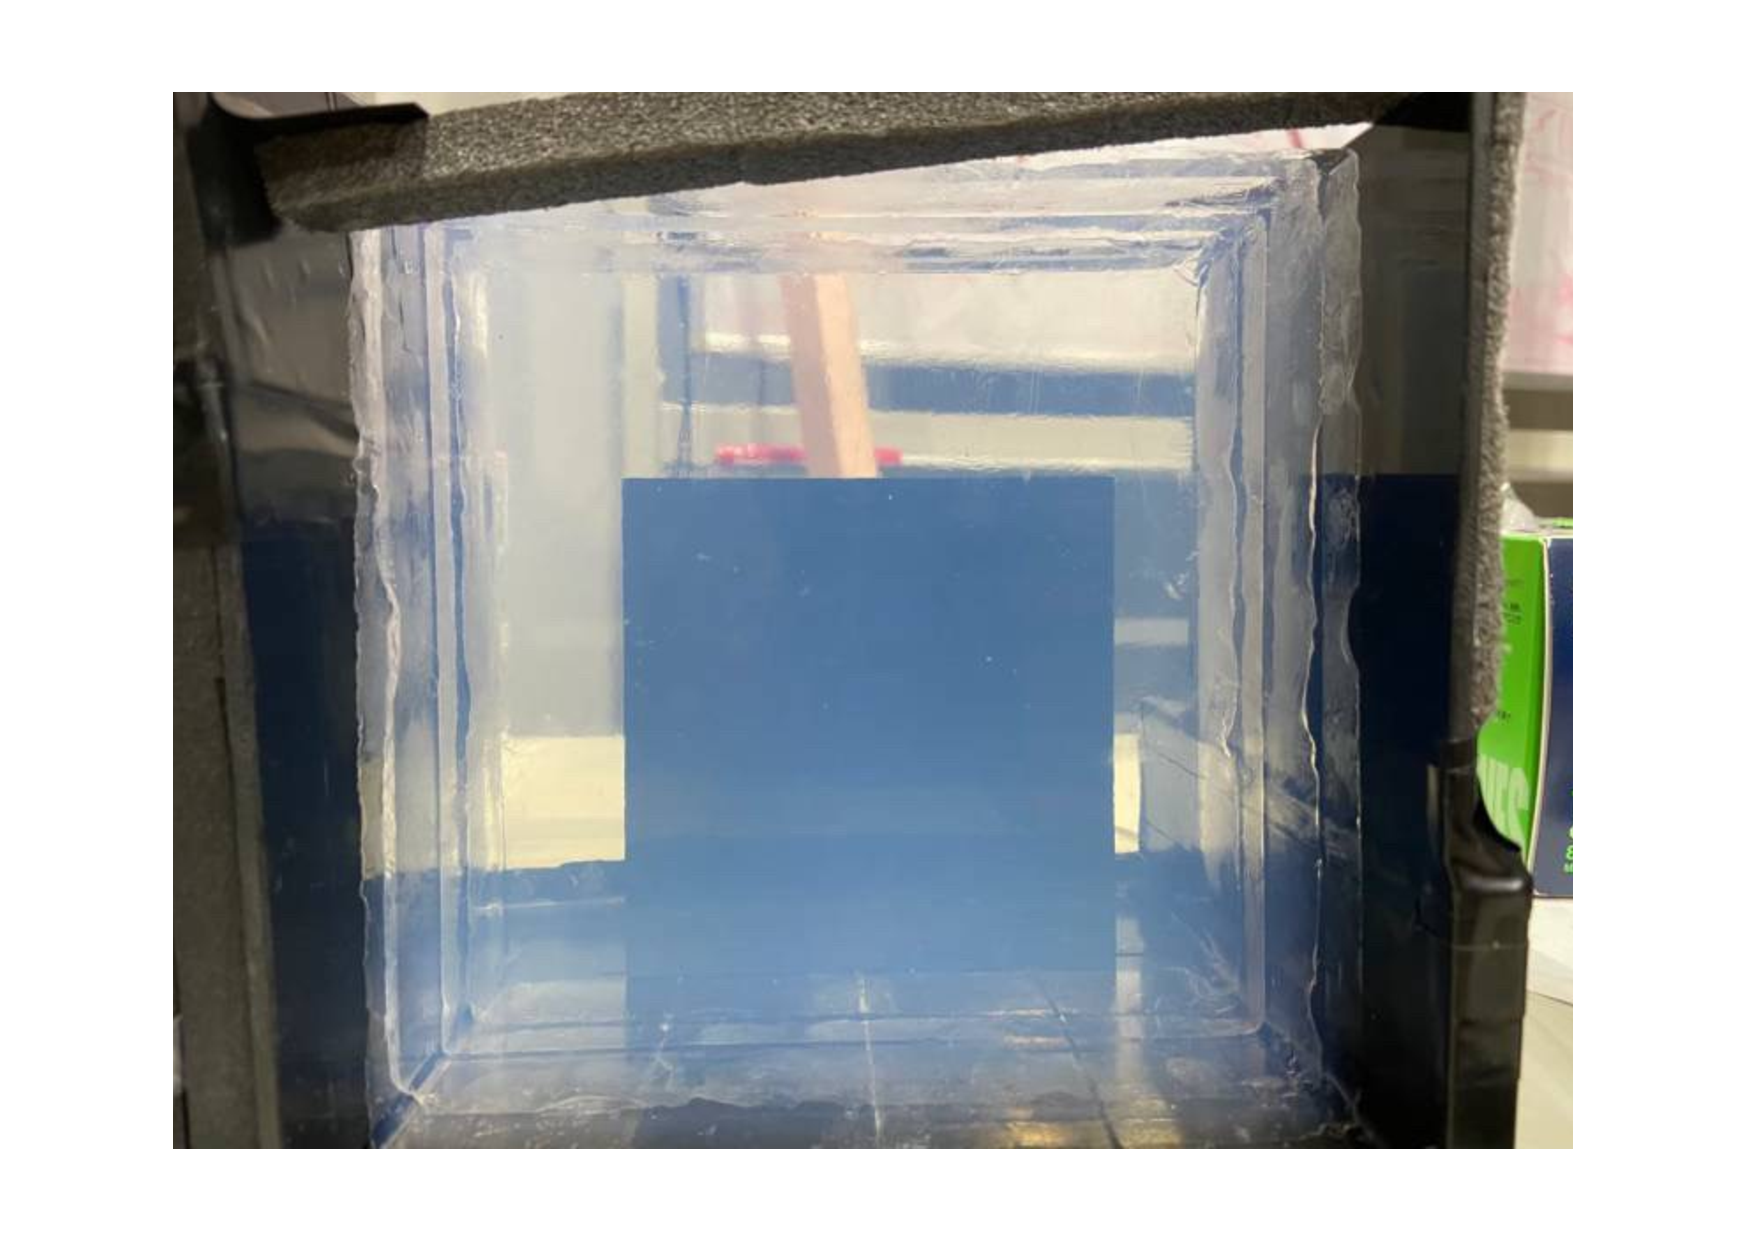
\includegraphics[width=10cm]{images/chapter3/Aerogel.pdf}
  \caption{使用したエアロゲルの写真。3つのエアロゲルを並べて厚さ$\SI{50}{mm}$として使用している。}
  \label{fig:Aerogle}
\end{figure}



\begin{table}[htbp]
  \caption{使用したエアロゲルのパラメータ}
  \label{table:Aerogel}
  \centering
  \begin{tabular}{cccc}
    \hline
    型番      & 屈折率    & 厚さ (mm) & 波長400 nmに対する透過長 (mm) \\
    \hline\hline
    TSA9-3  & 1.0400 & 20.7    & 54                   \\
    TSA10-3 & 1.0395 & 10.8    & 55                   \\
    TSA9-4  & 1.0397 & 21.0    & 58                   \\
    TSA40-1 & 1.0416 & 24.9    & 51.5                 \\
    TSA40-2 & 1.0412 & 25.0    & 50.6                 \\
    TSA40-3 & 1.0412 & 25.0    & 50.4                 \\
    TSA40-6 & 1.0411 & 25.0    & 50.4                 \\
    \hline
  \end{tabular}
\end{table}

\subsection{球面鏡}
図\ref{fig:Mirror}に使用した球面鏡の写真を示す。
球面鏡は四角の支えに四隅と各辺の真ん中を押さえて固定した。
支えの後ろには3つのボルトがついており、ボルトを出し縮みさせることで鏡の方向を調節できる様にした。
鏡のアライメントはエアロゲルの設置地点にレーザーを置き、鏡の中心で反射したレーザーが検出面の中心にくるように調整した。

\begin{figure}
  \centering
  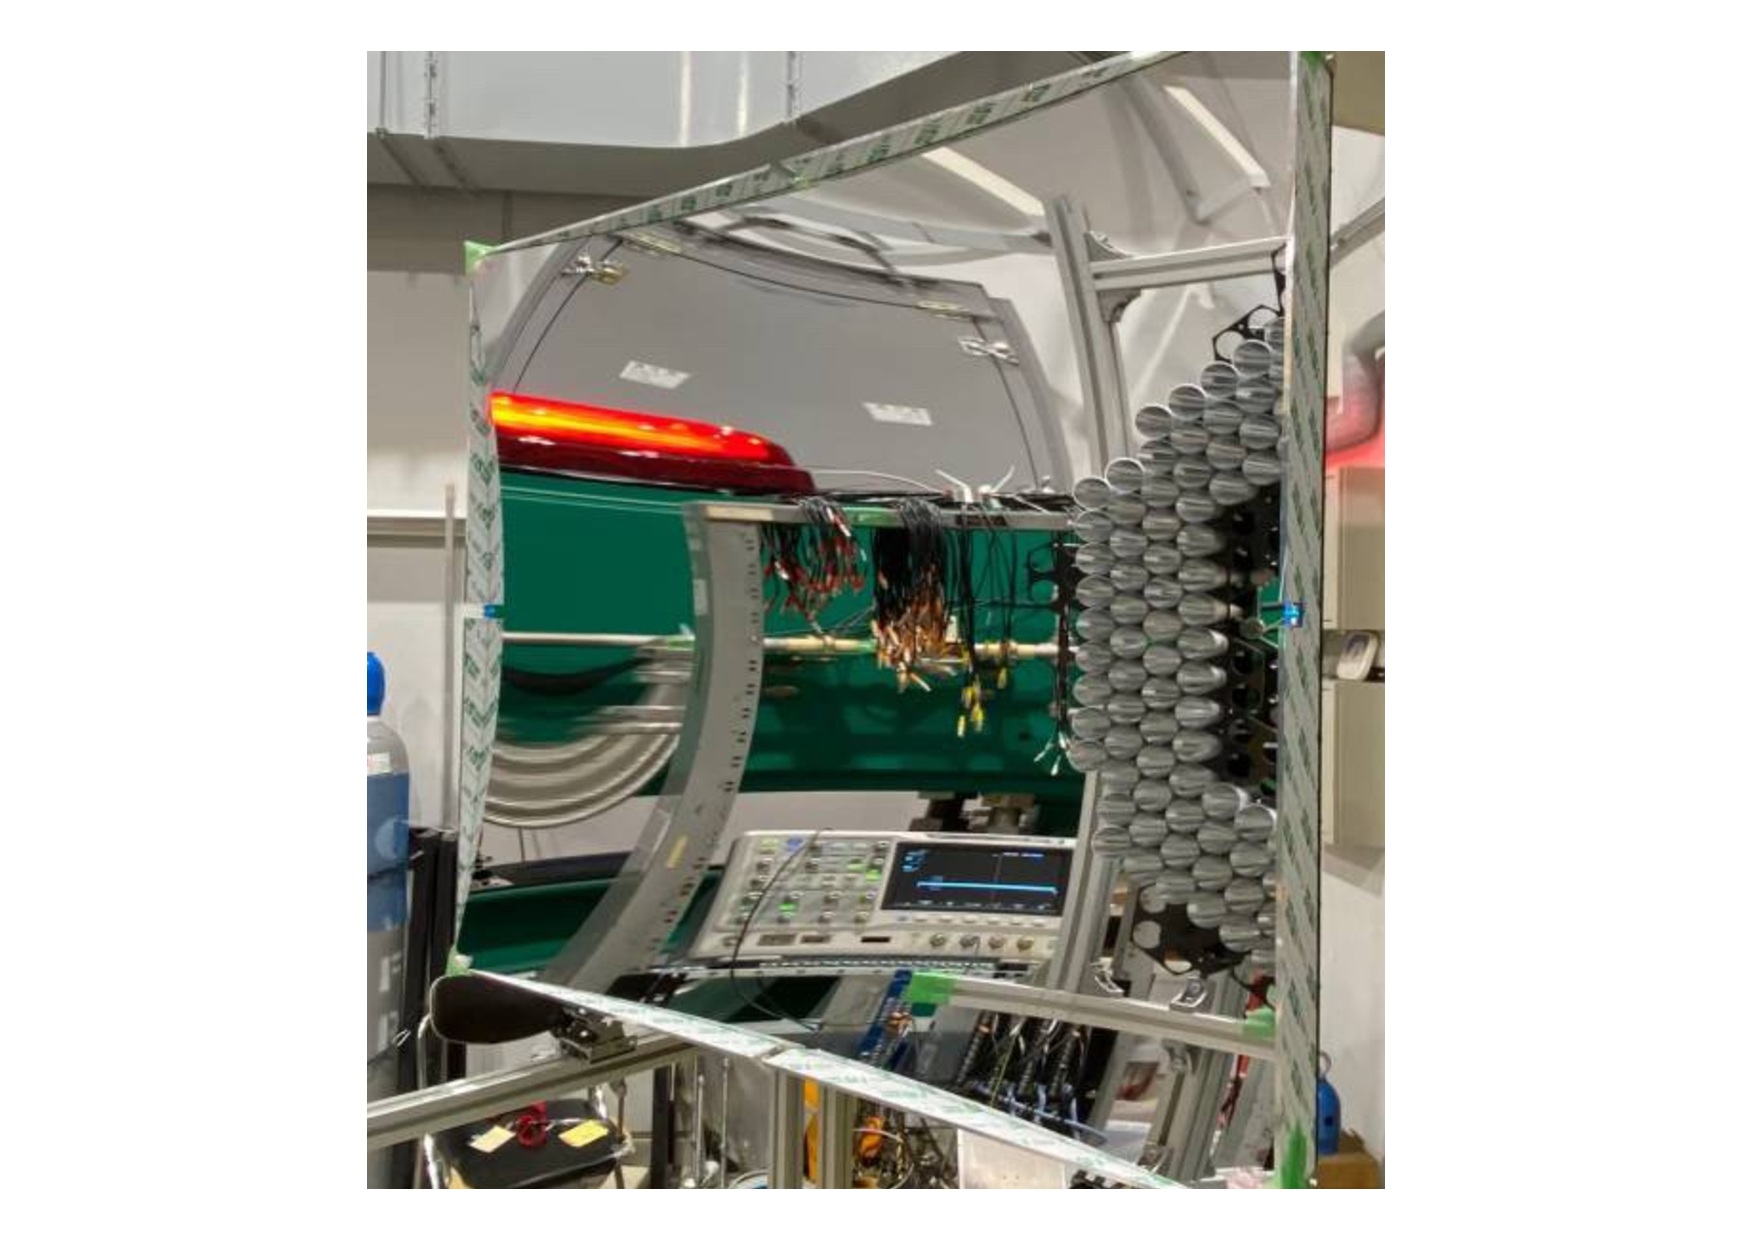
\includegraphics[width=10cm]{images/chapter3/Mirror.pdf}
  \caption{使用した$\SI{950}{mm}(縦)\times\SI{1080}{mm}(横)$の球面鏡の写真。}
  \label{fig:Mirror}
\end{figure}